\documentclass[a4paper,12pt,titlepage]{article}
\usepackage{amsmath} 
\usepackage{amssymb}
\usepackage[nottoc]{tocbibind}
\usepackage{mathrsfs}
\usepackage{float}
\usepackage{indentfirst}
\author{\textit{Jiang Yicheng}\\\textit{515370910224}}
\title{\textbf{VE203\\
		Assignment 9}}
\date{\today}
\usepackage{dsfont}
\usepackage[top=1in, bottom=1in, left= 1in, right=1in]{geometry}
\usepackage{fancyhdr,lastpage}
	\pagestyle{fancy}
	\fancyhf{}
\cfoot{Page \thepage\ of \pageref{LastPage}}
\usepackage{multirow}
\usepackage{gauss}
\usepackage[colorlinks=true,linkcolor=black]{hyperref}
\usepackage[linesnumbered,ruled,longend]{algorithm2e}
\SetKwInOut{Input}{Input}
\SetKwInOut{Output}{Output}
\newcommand{\To}{\KwTo}
\newcommand{\Ret}{\KwRet}
\SetKwProg{Fn}{Function}{\string:}{end}
\SetKwFunction{mc}{MC}
\newcommand{\udots}{\mathinner{\mskip1mu\raise1pt\vbox{\kern7pt\hbox{.}}\mskip2mu\raise4pt\hbox{.}\mskip2mu\raise7pt\hbox{.}\mskip1mu}}
\SetKwFunction{pow}{PowMod}
\usepackage{graphicx}
\usepackage{extarrows}
\usepackage{pdflscape}

\begin{document}

\maketitle

\section*{Exercise 9.1} 
\subsection*{i)}
\begin{figure}[H]
    \centering
    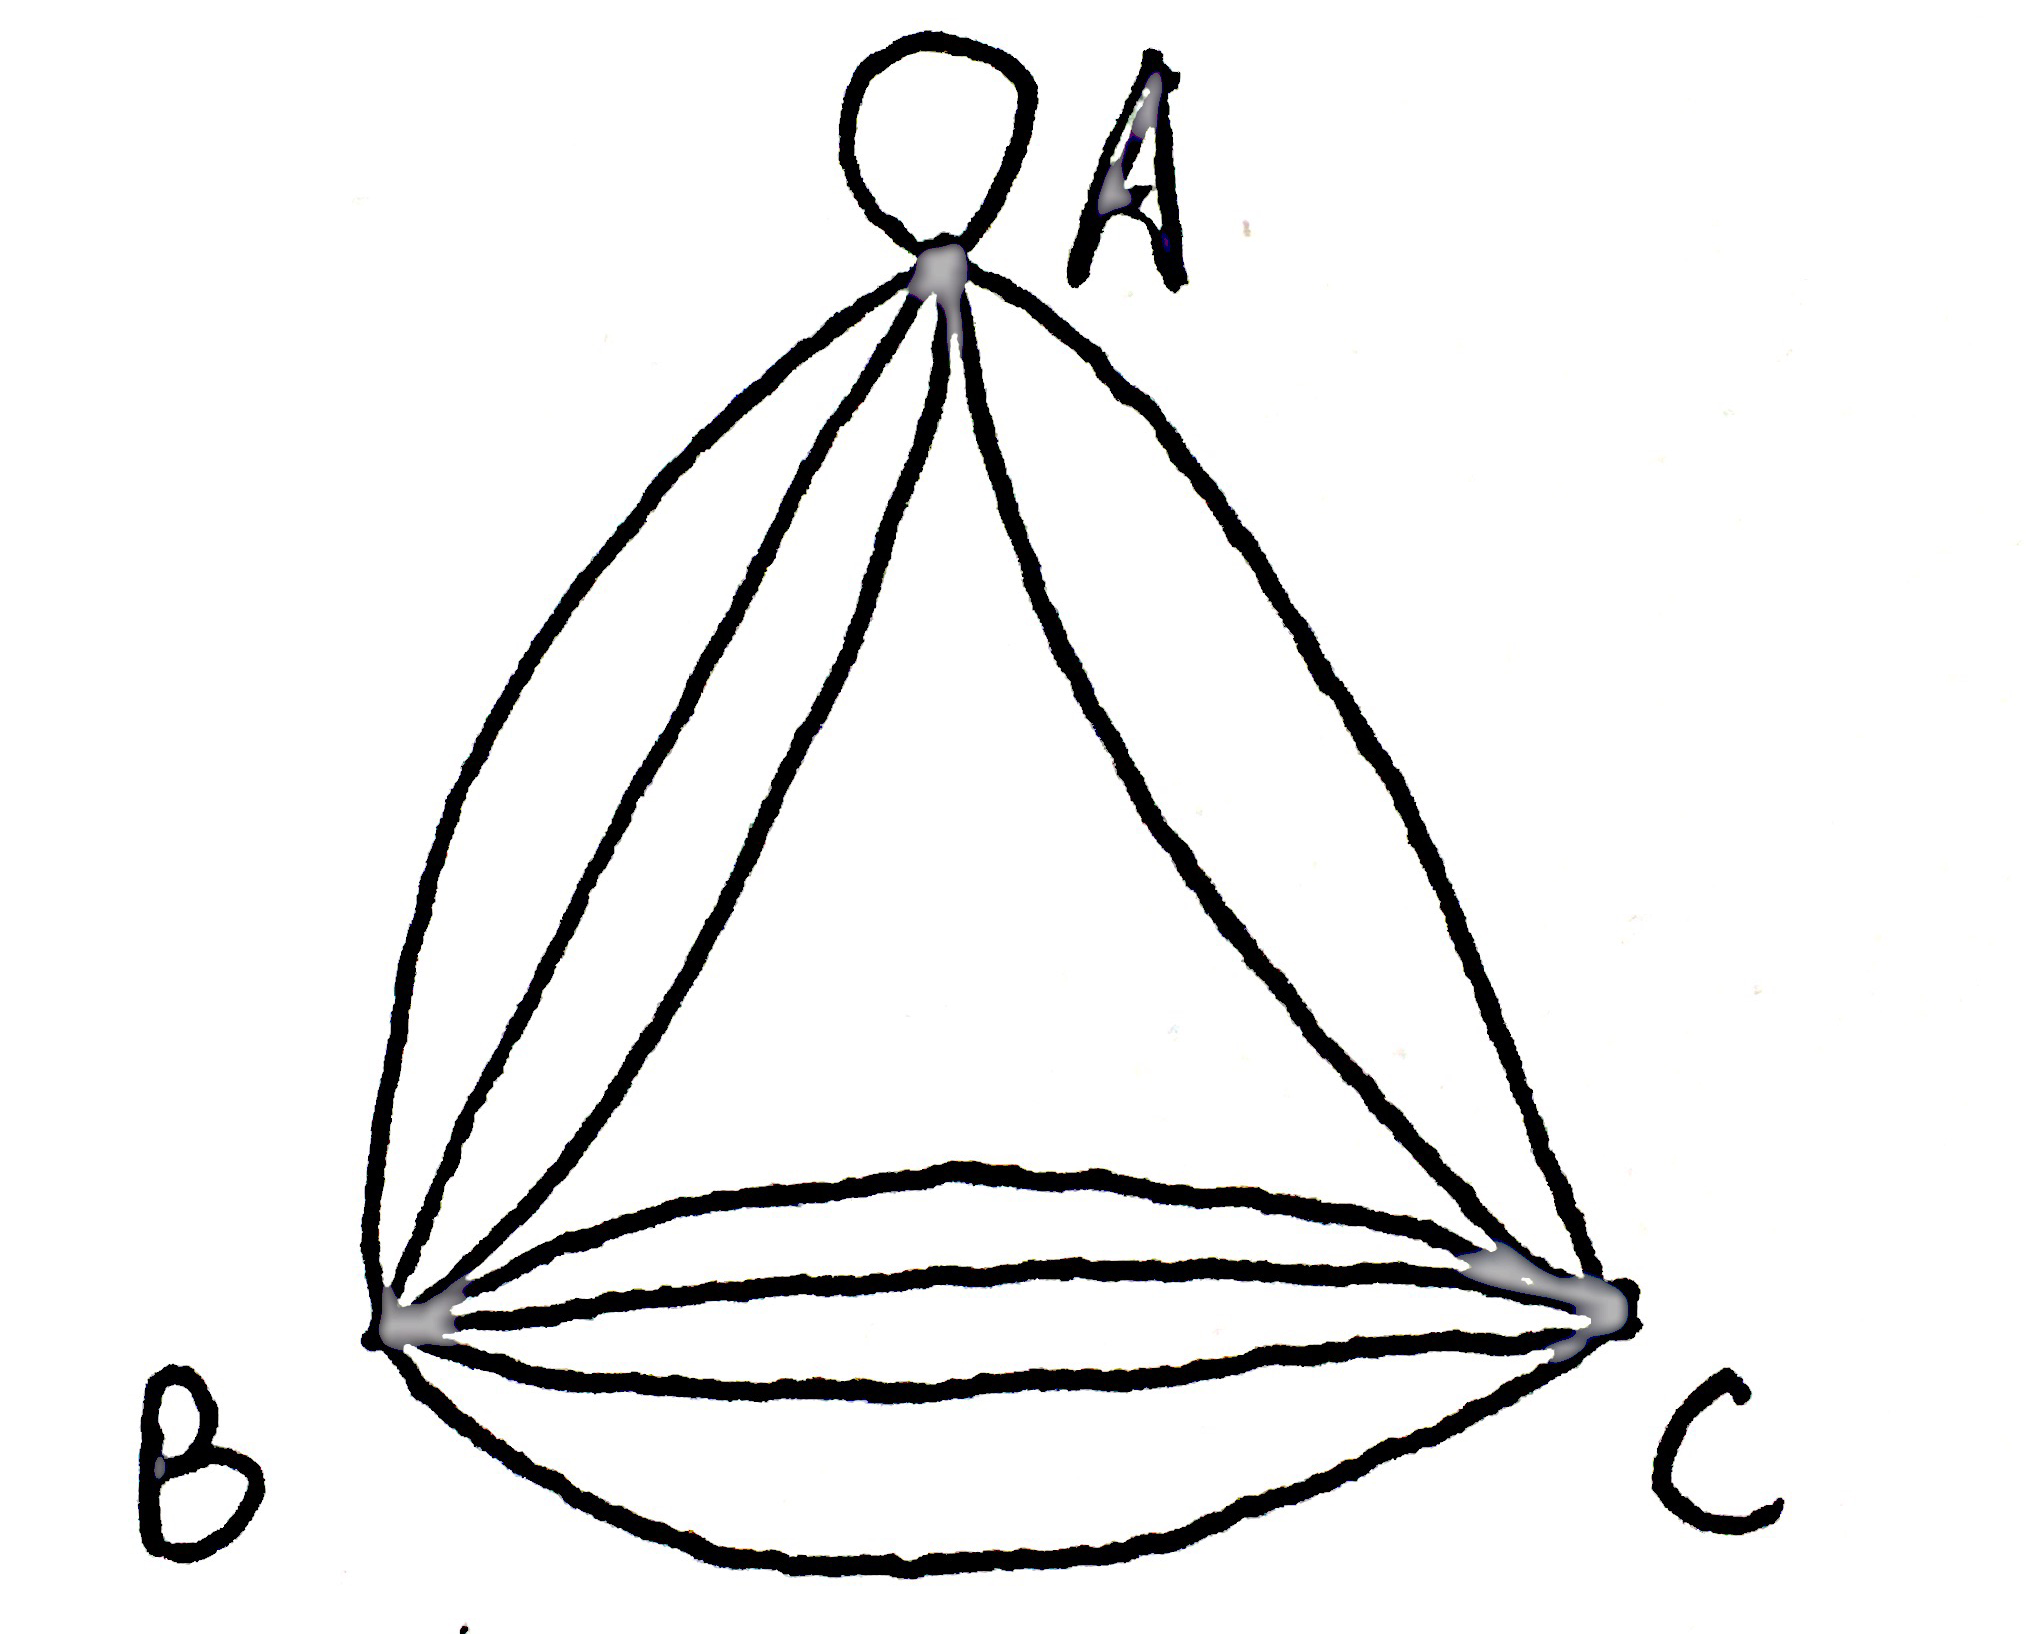
\includegraphics[width=7cm]{1.png}
\end{figure}
\subsection*{ii)}
\begin{figure}[H]
    \centering
    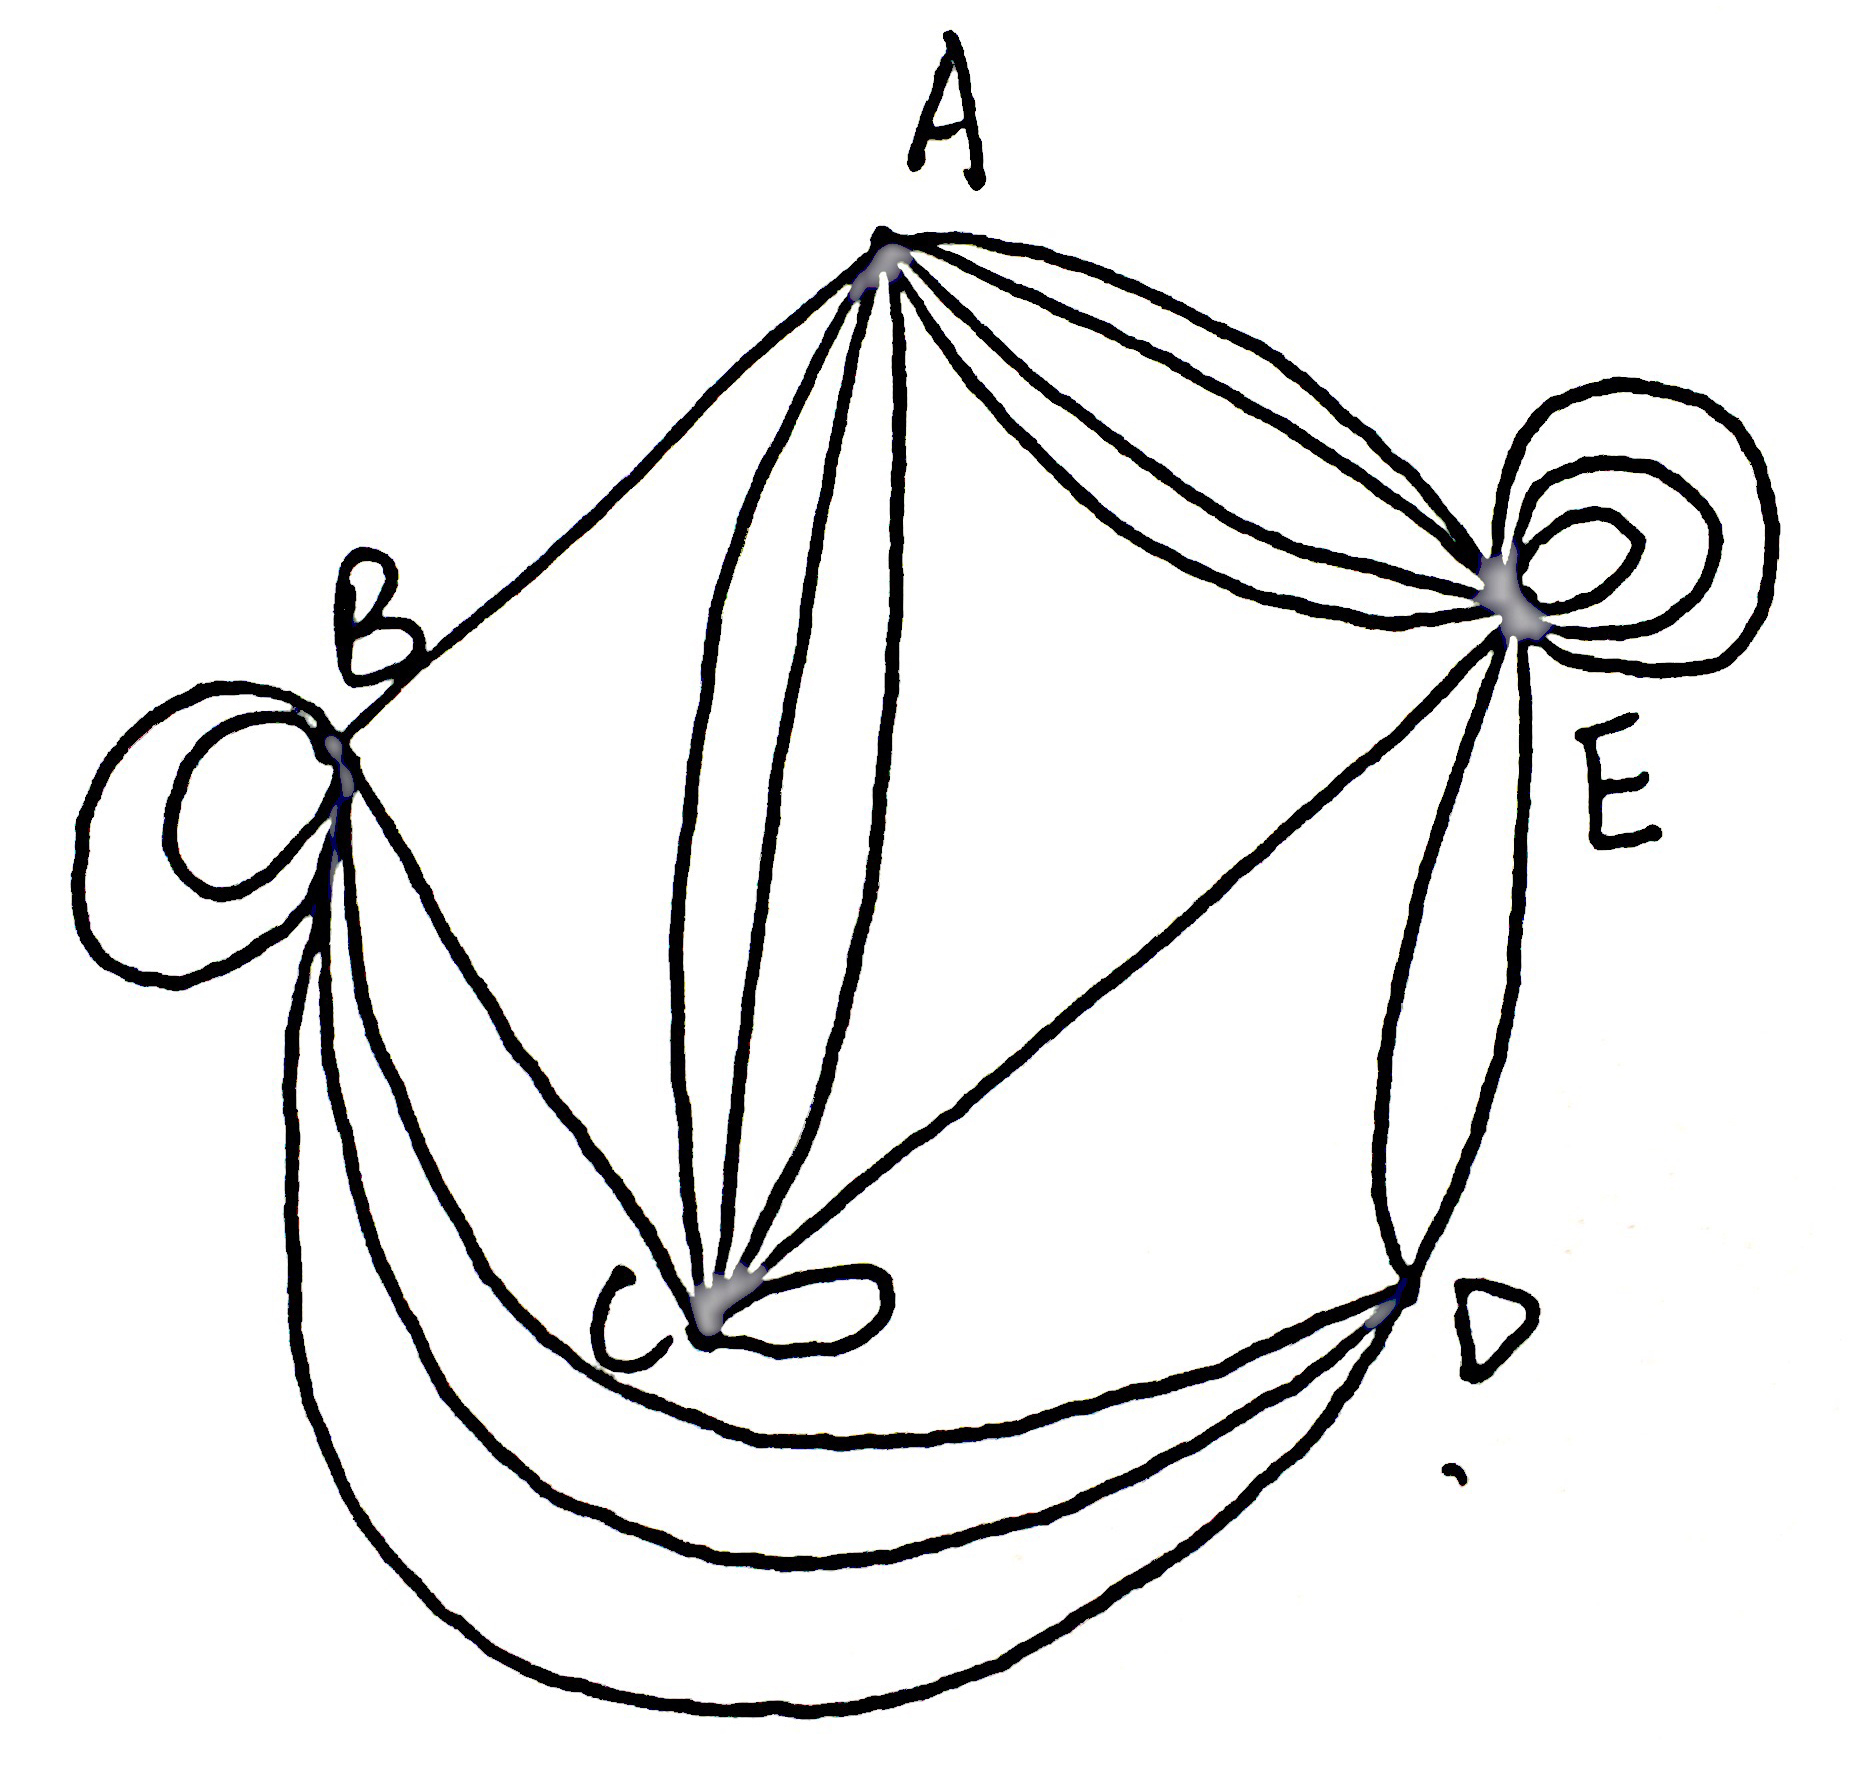
\includegraphics[width=7cm]{2.png}
\end{figure}
\section*{Exercise 9.2}
\subsection*{i)}
$$\varphi:u_1\mapsto v_1,u_2\mapsto v_3,u_3\mapsto v_5,u_4\mapsto v_2,u_5\mapsto v_4$$
Now $E=\lbrace \lbrace u_1,u_2\rbrace,\lbrace u_2,u_3\rbrace,\lbrace u_3,u_4\rbrace,\lbrace u_4,u_5\rbrace,\lbrace u_5,u_1\rbrace\rbrace$, so
\begin{align*}
\varphi* E=&\lbrace \lbrace \varphi(u_1),\varphi(u_2)\rbrace,\lbrace \varphi(u_2),\varphi(u_3)\rbrace,\lbrace \varphi(u_3),\varphi(u_4)\rbrace,\lbrace \varphi(u_4),\varphi(u_5)\rbrace,\lbrace \varphi(u_5),\varphi(u_1)\rbrace\rbrace\\
=&\lbrace \lbrace v_1,v_3\rbrace,\lbrace v_3,v_5\rbrace,\lbrace v_5,v_2\rbrace,\lbrace v_2,v_4\rbrace,\lbrace v_4,v_1\rbrace\rbrace\\
=&F
\end{align*}
So the given pair of graphs is isomorphic.
\subsection*{ii)}
$$\varphi:u_3\mapsto v_2,u_2\mapsto v_3,u_1\mapsto v_4,u_5\mapsto v_1,u_4\mapsto v_5$$
Now $E=\lbrace \lbrace u_1,u_2\rbrace,\lbrace u_1,u_4\rbrace,\lbrace u_1,u_5\rbrace,\lbrace u_2,u_5\rbrace,\lbrace u_2,u_4\rbrace,\lbrace u_2,u_3\rbrace,\lbrace u_3,u_4\rbrace,\lbrace u_4,u_5\rbrace\rbrace$, so
\begin{align*}
\varphi* E=&\lbrace \lbrace \varphi(u_1),\varphi(u_2)\rbrace, \lbrace \varphi(u_1),\varphi(u_4)\rbrace, \lbrace \varphi(u_1),\varphi(u_5)\rbrace, \lbrace \varphi(u_2),\varphi(u_5)\rbrace,\lbrace \varphi(u_2),\varphi(u_4)\rbrace,\\&\lbrace \varphi(u_2),\varphi(u_3)\rbrace,\lbrace \varphi(u_3),\varphi(u_4)\rbrace,\lbrace \varphi(u_4),\varphi(u_5)\rbrace\rbrace\\
=&\lbrace \lbrace v_4,v_3\rbrace,\lbrace v_4,v_5\rbrace,\lbrace v_4,v_1\rbrace,\lbrace v_3,v_1\rbrace,\lbrace v_3,v_5\rbrace,\lbrace v_3,v_2\rbrace,\lbrace v_2,v_5\rbrace,\lbrace v_5,v_1\rbrace\rbrace\\
=&F
\end{align*}
So the given pair of graphs is isomorphic.
\subsection*{iii)}
\begin{equation*} 
A=\begin{array}{c}
\\
v_1\\
v_2\\
v_3\\
v_4\\
v_5\\
v_6\\
v_7\\
v_8
\end{array} 
\begin{array}{c}   
    v_1\,\, v_2 \,\,\, v_3 \,\, v_4 \,\, v_5 \,\, v_6\,\, v_7\,\, v_8 \\
  \left(                 
  \begin{array}{cccccccc}   
    0 & 1 & 0 & 0 & 0 & 1 & 0 & 1 \\  
    1 & 0 & 1 & 0 & 1 & 0 & 0 & 0 \\
    0 & 1 & 0 & 1 & 0 & 0 & 0 & 1 \\
    0 & 0 & 1 & 0 & 1 & 0 & 1 & 0 \\
    0 & 1 & 0 & 1 & 0 & 1 & 0 & 0 \\
    1 & 0 & 0 & 0 & 1 & 0 & 1 & 0 \\
    0 & 0 & 0 & 1 & 0 & 1 & 0 & 1 \\
    1 & 0 & 1 & 0 & 0 & 0 & 1 & 0 \\
  \end{array}
\right)  
\end{array}    
A^3=\begin{array}{c}
\\
v_1\\
v_2\\
v_3\\
v_4\\
v_5\\
v_6\\
v_7\\
v_8
\end{array} 
\begin{array}{c}   
    v_1\,\, v_2 \,\,\, v_3 \,\, v_4 \,\, v_5 \,\, v_6\,\, v_7\,\, v_8 \\
  \left(                 
  \begin{array}{cccccccc}   
    0 & 7 & 0 & 6 & 0 & 7 & 0 & 7 \\  
    7 & 0 & 7 & 0 & 7 & 0 & 6 & 0 \\
    0 & 7 & 0 & 7 & 0 & 6 & 0 & 7 \\
    6 & 0 & 7 & 0 & 7 & 0 & 7 & 0 \\
    0 & 7 & 0 & 7 & 0 & 7 & 0 & 6 \\
    7 & 0 & 6 & 0 & 7 & 0 & 7 & 0 \\
    0 & 6 & 0 & 7 & 0 & 7 & 0 & 7 \\
    7 & 0 & 7 & 0 & 6 & 0 & 7 & 0 \\
  \end{array}
\right)  
\end{array}   
\end{equation*}
So we can see that in the second graph there doesn't exist a length 3 circuit. While in the first graph, we can see that $u_2\rightarrow u_3\rightarrow u_1\rightarrow u_2$ is a length three circuit. So we can see that the given pair of graphs is  not isomorphic.


\subsection*{iv)}
$$\varphi:u_2\mapsto v_1,u_6\mapsto v_8,u_4\mapsto v_4,u_8\mapsto v_5,u_3\mapsto v_3,u_5\mapsto v_7,u_1\mapsto v_2,u_7\mapsto v_6$$
Now $E=\lbrace \lbrace u_1,u_2\rbrace,\lbrace u_1,u_3\rbrace,\lbrace u_1,u_8\rbrace,\lbrace u_2,u_3\rbrace,\lbrace u_2,u_6\rbrace,\lbrace u_3,u_4\rbrace,\lbrace u_4,u_5\rbrace,\lbrace u_4,u_8\rbrace,\\\lbrace u_5,u_6\rbrace,\lbrace u_5,u_7\rbrace,\lbrace u_6,u_7\rbrace,\lbrace u_7,u_8\rbrace\rbrace$, so
\begin{align*}
\varphi* E=&\lbrace \lbrace \varphi(u_1),\varphi(u_2)\rbrace, \lbrace \varphi(u_1),\varphi(u_3)\rbrace, \lbrace \varphi(u_1),\varphi(u_8)\rbrace, \lbrace \varphi(u_2),\varphi(u_3)\rbrace,\lbrace \varphi(u_2),\varphi(u_6)\rbrace,\\&\lbrace \varphi(u_3),\varphi(u_4)\rbrace,\lbrace \varphi(u_4),\varphi(u_5)\rbrace,\lbrace \varphi(u_4),\varphi(u_8)\rbrace,\lbrace \varphi(u_5),\varphi(u_6)\rbrace,\lbrace \varphi(u_5),\varphi(u_7)\rbrace,\\
&\lbrace \varphi(u_6),\varphi(u_7)\rbrace,\lbrace \varphi(u_7),\varphi(u_8)\rbrace\rbrace\\
=&\lbrace \lbrace v_2,v_1\rbrace,\lbrace v_2,v_3\rbrace,\lbrace v_2,v_5\rbrace,\lbrace v_1,u_3\rbrace,\lbrace v_1,v_8\rbrace,\lbrace v_3,v_4\rbrace,\lbrace v_4,v_7\rbrace,\lbrace v_4,v_5\rbrace,\\
&\lbrace v_7,v_8\rbrace,\lbrace v_7,v_6\rbrace,\lbrace v_8,v_6\rbrace,\lbrace v_6,v_5\rbrace\rbrace\\
=&F
\end{align*}
So the given pair of graphs is isomorphic.
\section*{Exercise 9.3}
\subsection*{i)}
For $n$ is even and $n>2$, the degree of each vertex is $n-1$ which is odd. So there are more than two vertices whose degree are odd in $K_n$ and therefore it doesn't have an Euler circuit. For $n=2$, it doesn't have an Euler circuit obviously.

For $n$ is odd, the degree of each vertex is $n-1$ which is even. For $n=1$, since there is only one vertex and no edge, there are no path and therefore it doesn't have an Euler circuit.  For $n\geqslant3$, $K_n$ is connected and all vertices' degree are even  and therefore it has an Euler circuit. 

To sum up, for $n=2k+1,k\geqslant1,k\in\mathbb{Z}$, $K_n$ has an Euler circuit.

\section*{ii)}
$\forall n\geqslant3$, $W_n$ has $n$ vertices whose degree are three and therefore it doesn't have an Euler circuit.

To sum up, $\forall n\geqslant3$, $W_n$ doesn't have an Euler circuit.
\section*{iii)}
$\forall n\geqslant3$, $C_n$ has an obvious Euler circuit according to its definition.
\section*{iv)}
For $n$ is even and $n$, $Q_n$ is connected and the degree of each vertex is $n$ which is even and therefore $Q_n$ has an Euler circuit.

For $n$ is odd, the degree of each vertex is $n$ which is odd. For $n=1$, since it is just $K_2$ and therefore it doesn't have an Euler circuit. For $n\geqslant3$, $Q_n$ has $2^n>3$ vertices whose degree are odd and therefore it doesn't have an Euler circuit. 

To sum up, for $n=2k,k\geqslant1,k\in\mathbb{Z}$, $Q_n$ has an Euler circuit.
\section*{Exercise 9.4}
We first prove that if all simple circuits have even length, then the graph with at least two vertices is bipartite.

For two vertices $u$ and $v$, let the distance $d(u, v)$ be the length of the shortest path joining $u$ to $v$. Then choose an arbitrary vertex $u$ and setting $S = \lbrace v : 2 | d(u, v)\rbrace$ and $T =\lbrace v : 2 \nmid d(u, v)\rbrace$.

$\forall x,y\in S$, if $d(x,y)=1$, then $x,y\neq u$ and  $d(x,y)+d(x,u)+d(y,u)$ is odd since $d(x,u),d(y,u)$ are both even. This means that the length of a simple circuit from $u$ to $u$ contains $x,y$ is odd. This leads contradiction to the given qualification that all simple circuits have even length. So $d(x,y)\neq1$. $\forall x,y\in T$, this is also true.

$\forall x\in S,y\in T$, if $d(x,y)=1$ then they have different color. So, for any two vertices $x,y$, if $d(x,y)=1$, then they have different colors. So the graph is bipartite.

Now we try to prove that if a graph is bipartite, then all simple circuits have even length.

For any simple circuit, it starts from one vertex and end at the same vertex. Since the graph is bipartite, when the circuit goes from one vertex to its next vertex, the length will increase by 1 and the circuit goes from one color to the other color. So when the circuit goes into a vertex with different color, the parity of the length of the circuit will change. Since circuit starts from one vertex and end at the same vertex, the parity won't change and keep even. So all simple circuits have even length.

To sum up, a graph with at least two vertices is bipartite if and only if all simple circuits have even length.

\section*{Exercise 9.5}
The hypercube $Q_n$ bipartite for all $n \in \mathbb{N}$.

We can choose one vertex $u$ and divide all verticles into two parts: if bit strings of one vertex differ from $u's$ in even digits, they are in set $S$, if they differ odd digits, they are in set $T$. 

$\forall x,y\in S$, since $x,y$ differ from $u's$ bit string by even digits, the bit srings of $x,y$ differ from even digits and they are not connected with each other. $\forall x,y\in T$, this is also true.

So according to our construction, two connected verticles must have different colors. And therefore $Q_n$ is bipartite for all $n\in\mathbb{N}$.

\section*{Exercise 9.6}
\subsection*{i)}
If a simple graph $G$ is a self-complementary graph, then $G$ and $G^c$ must have the same number of edges. So hte total number of edges of $G$ and $G^c$ is even. Set $G$ has $n$ vertices, then $a:=\begin{pmatrix}
n\\
2
\end{pmatrix}=\dfrac{n(n-1)}{2}
$
is even.
\begin{enumerate}
\item If $n=4m,m\in\mathbb{N}^*$, $a=2m(4m-1)$ is even.
\item If $n=4m+1,m\in\mathbb{N}^*$, $a=2m(4m+1)$ is even.
\item If $n=4m+2,m\in\mathbb{N}$, $a=(2m+1)(4m+1)$ is odd.
\item If $n=4m+3,m\in\mathbb{N}$, $a=(4m+3)(2m+1)$ is odd.
\end{enumerate}
So $a$ is even if and only if $n=4m\vee n=4m+1,m\in\mathbb{N}^*$. Also for $m=0$ we can see the statement is also true. So a self-complementary graph must have either $4m$ or $4m + 1$ vertices, $m\in\mathbb{N}$.

\subsection*{ii)}
\begin{enumerate}
\item $n=0$
\item $n=1$
$$\bullet$$
\item $n=4$
\begin{figure}[H]
    \centering
    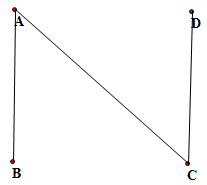
\includegraphics[width=7cm]{84.png}
\end{figure}
\item $n=5$
\begin{figure}[H]
    \centering
    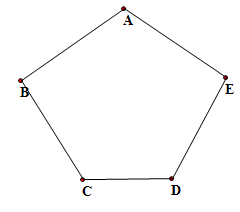
\includegraphics[width=7cm]{851.png}
\end{figure}
\begin{figure}[H]
    \centering
    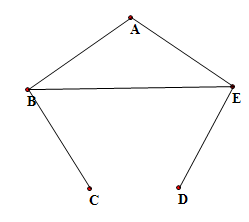
\includegraphics[width=7cm]{852.png}
\end{figure}
\item $n=8$
\begin{figure}[H]
    \centering
    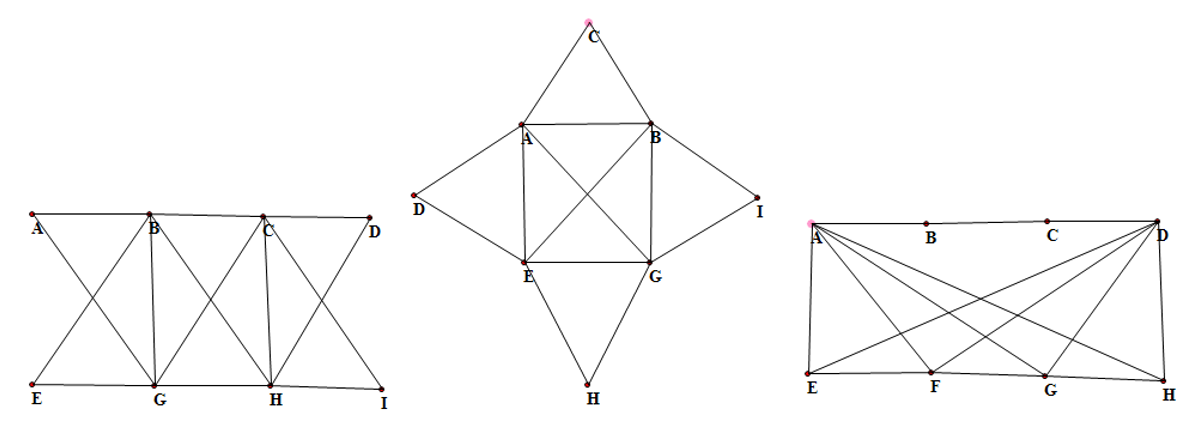
\includegraphics[width=12cm]{81.png}
\end{figure}
\begin{figure}[H]
    \centering
    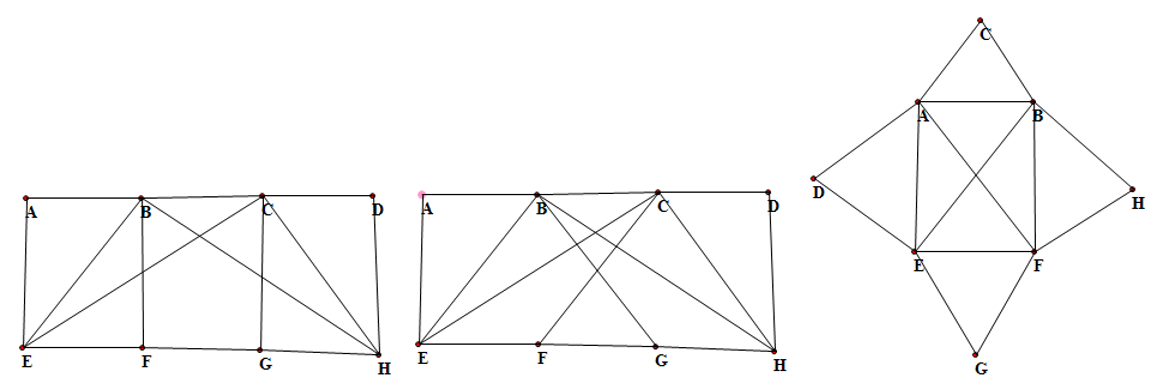
\includegraphics[width=12cm]{82.png}
\end{figure}
\begin{figure}[H]
    \centering
    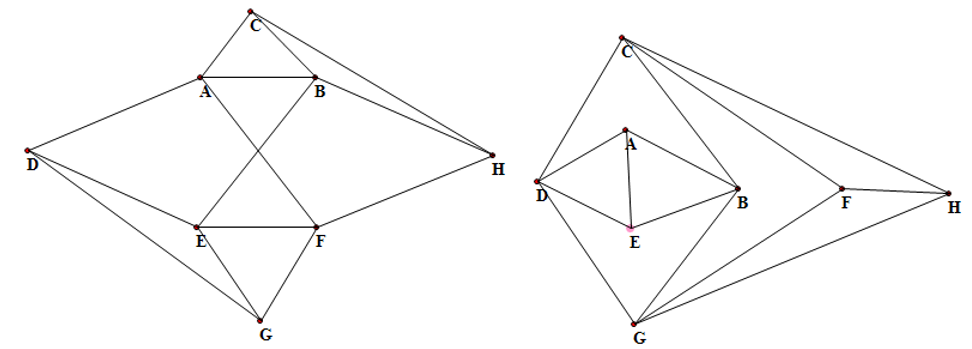
\includegraphics[width=12cm]{83.png}
\end{figure}
\begin{figure}[H]
    \centering
    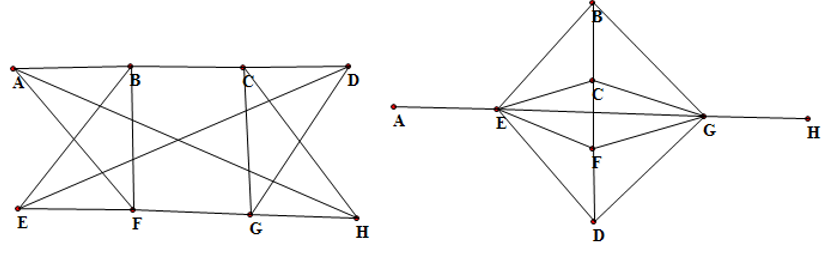
\includegraphics[width=12cm]{841.png}
\end{figure}
\end{enumerate}
\section*{Exercise 9.7}
\subsection*{i)}
Set $G$ has $n$ vertices, we define $H$ as $K_n\setminus\lbrace e_1\rbrace$ where $e_1$ is an arbitrary edge in $K_n$. Then when add an edge to $H$, it becomes $K_n$ and therefore there must exist a Hamilton circuit. So there exists another graph $H$ with the same vertices as $G$, which can be constructed by adding edges to $G$ such that the addition of a single edge would produce a Hamilton circuit in $H$. 
 
\subsection*{ii)}
Since when add an edge to $H$ there exist a Hamilton circuit, then we delete the added edge $e_1$ and reutrn to $H$:
\begin{enumerate}
\item If $e_1$ isn't contained in the Hamilton circuit, then the circuit hasn't been destroyed and therefore there is a Hamilton path in $H$.

\item If $e_1$ is contained in the Hamilton circuit, then we choose one vertex of $e_1$ to be the starting vertex and the other one to be the end point and it is a Hamilton path in $H$.
\end{enumerate}
So there is a Hamilton path in H.
\subsection*{iii)}
The number of vertices not adjacent to $v_n$ is at most
$$a:=n-1-deg(v_n)+1$$
Since $deg(v_1)+deg(v_n)>n$, 
$$a=n-deg(v_n)<deg(v_1)$$
So there are at most $deg(v_1)$ vertices not adjacent to $v_n$. 

\subsection*{iv)}
Since $v_1,v_2,\cdots,v_n$ is a Hamilton path in $H$, then all vertex adjacent to $v_1$ is among these verteices and therefore $S$ contains deg$(v_1)$ vertices. And $v_n\notin S$ otherwise the Hamilton path becomes Hamilton circuit.    

\subsection*{v)}
Since there here are at most $deg(v_1)$ vertices not adjacent to $v_n$ include $v_n$ itself and $v_n\notin S$, among the $deg(v_1)$ vertices in $S$, there must exist at least one vertex $v_k\in S$, which is adjacent to $v_n$.  So there are edges connecting $v_1$ and $v_{k+1}$ and $v_k$ and $v_n$.

\subsection*{vi)}
From former questions, we can conclude that $v_1,v_2,\cdots,v_{k-1},v_k,v_n,v_{n-1},\cdots,v_{k+1},v_1$ is a Hamilton circuit in $G$. And therefore the Ore's Theorem holds.
\clearpage


\section*{Exercise 9.8}

\begin{figure}[H]
    \centering
    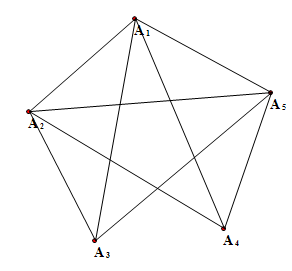
\includegraphics[angle=90,height=21.5cm]{8.png}
\end{figure}
For the vertices don't appear in the table, their labels keep $\infty$ to the end. So $S_k=\lbrace U,Z,P,S,Y\rbrace$ and the shortest path between Tiantong Rd. station and Zhaojiabang Rd. station is 23.





\end{document}
